\label{appendix:a}

\begin{figure}
\centering
\text{Latent space encodings for the Windy Slope scenario.}
\captionsetup{size=footnotesize}
\begin{subfigure}{\linewidth}
  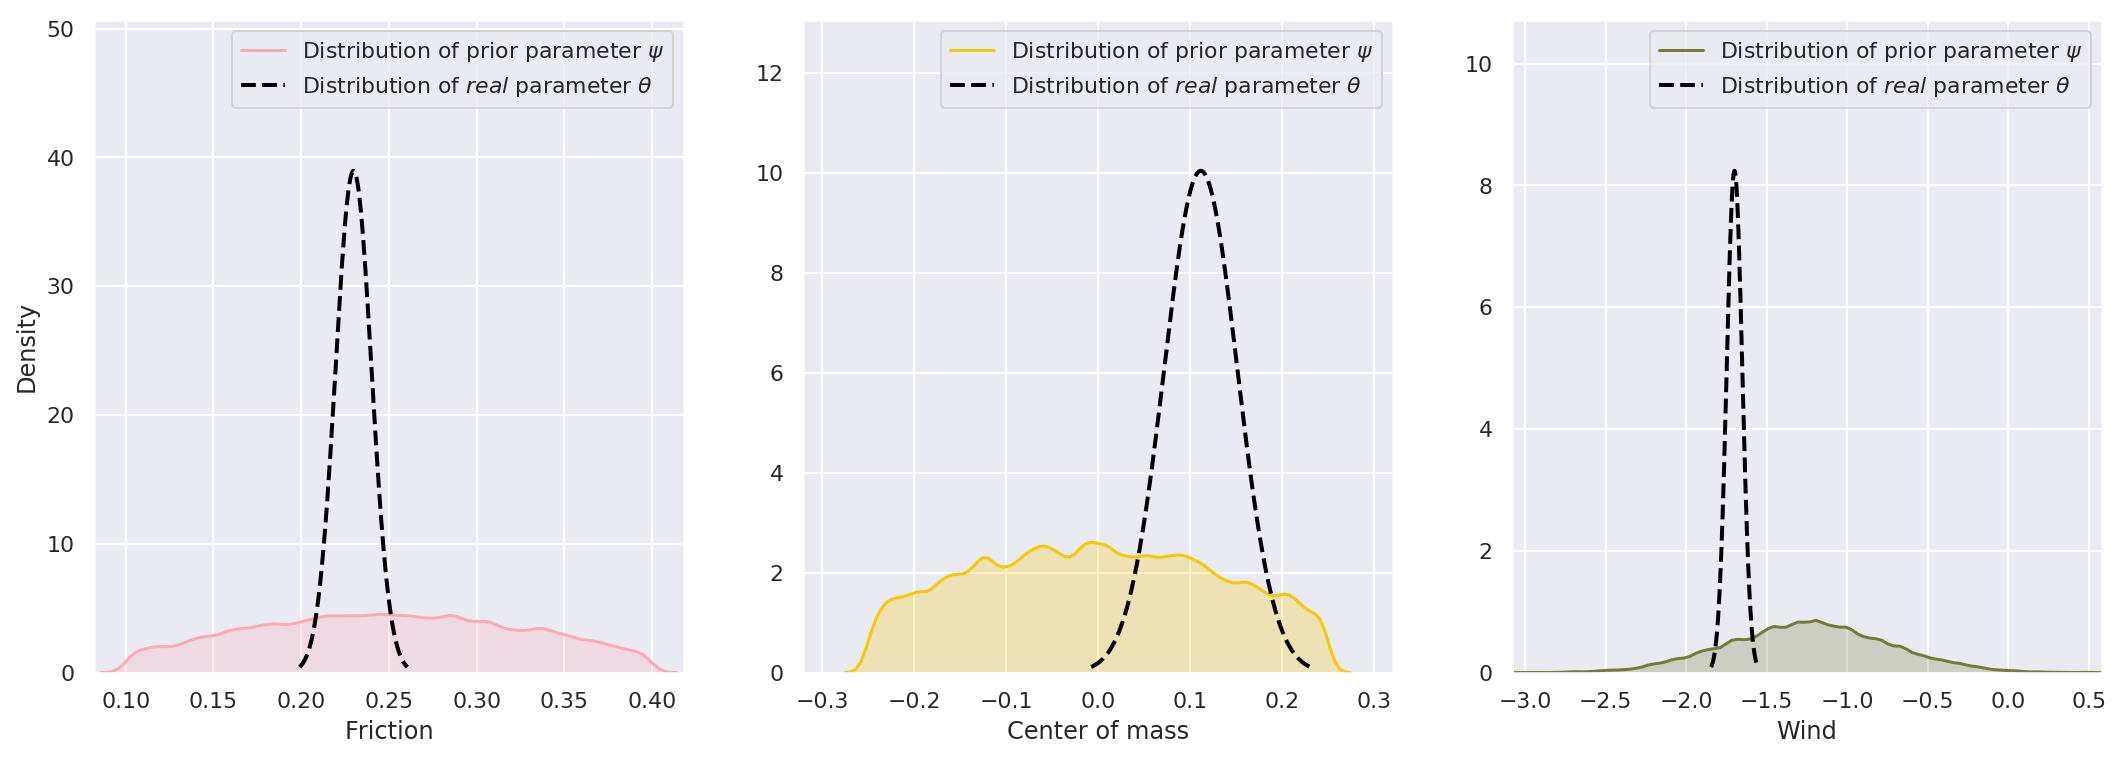
\includegraphics[width=1.0\linewidth]{img/windyslope/latent-representation/new/iter0}
  \caption{Initial estimates of $\psi$}
  \label{fig_3_parameters_0}
\end{subfigure}
\begin{subfigure}{\linewidth}
  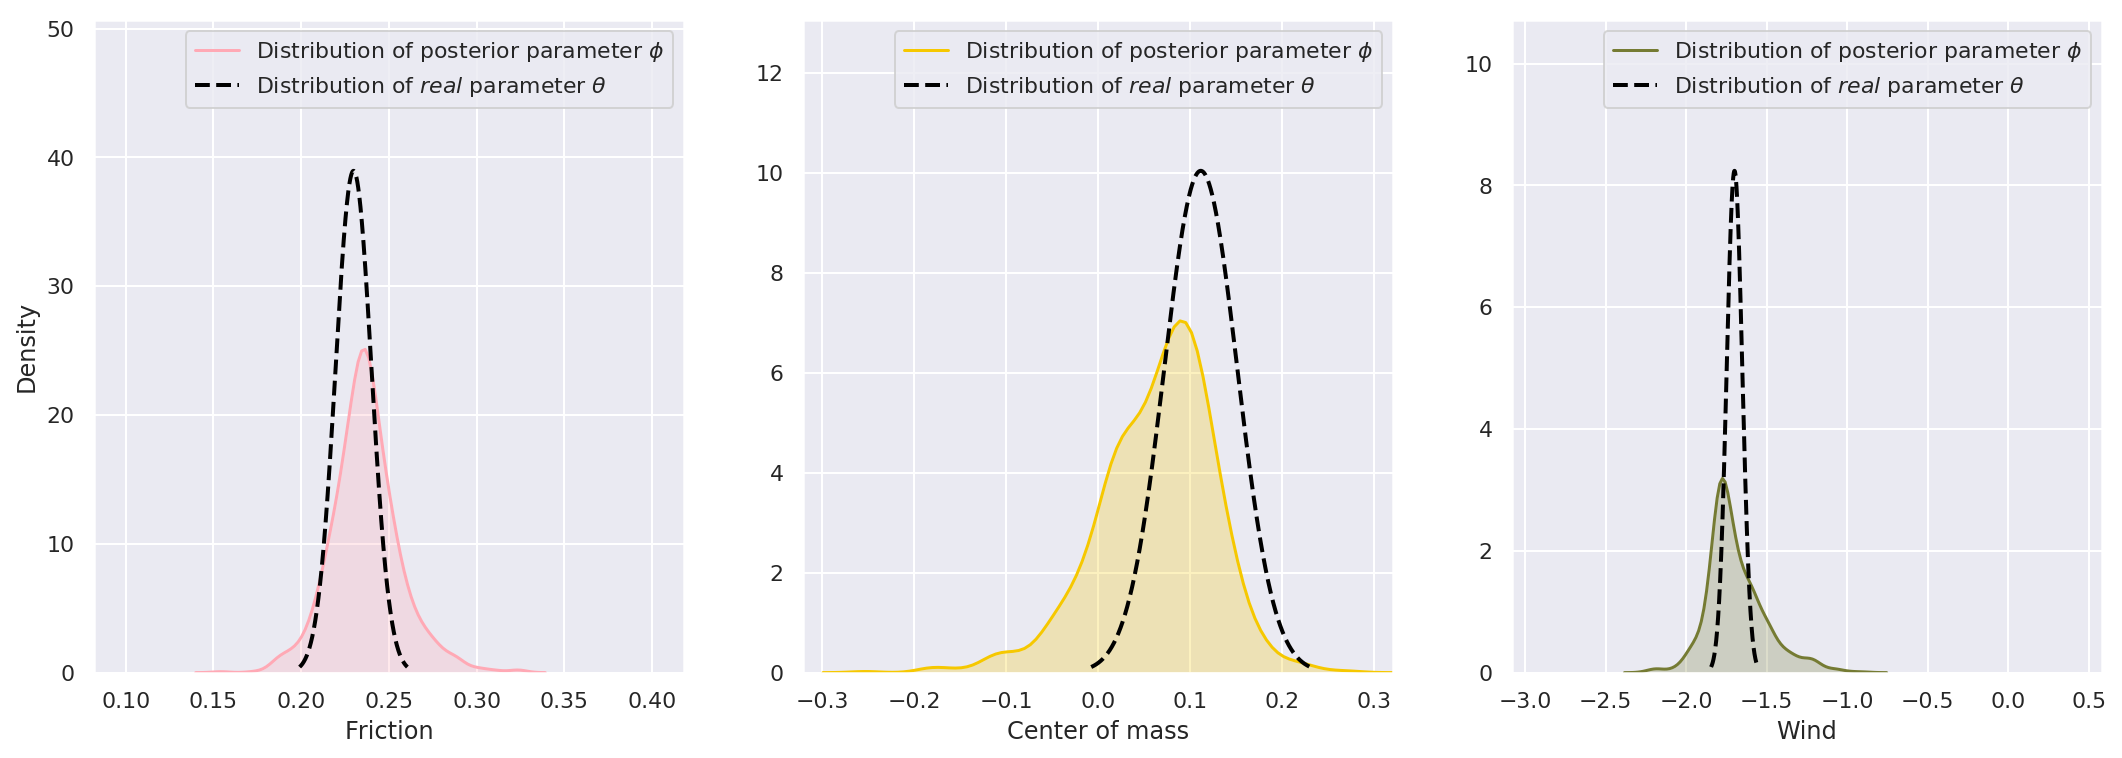
\includegraphics[width=1.0\linewidth]{img/windyslope/latent-representation/new/latent_encoding_iter1}
  \caption{1st iteration of \dettostoc{}}
  \label{fig_3_parameters_0}
\end{subfigure}
\begin{subfigure}{\textwidth}
  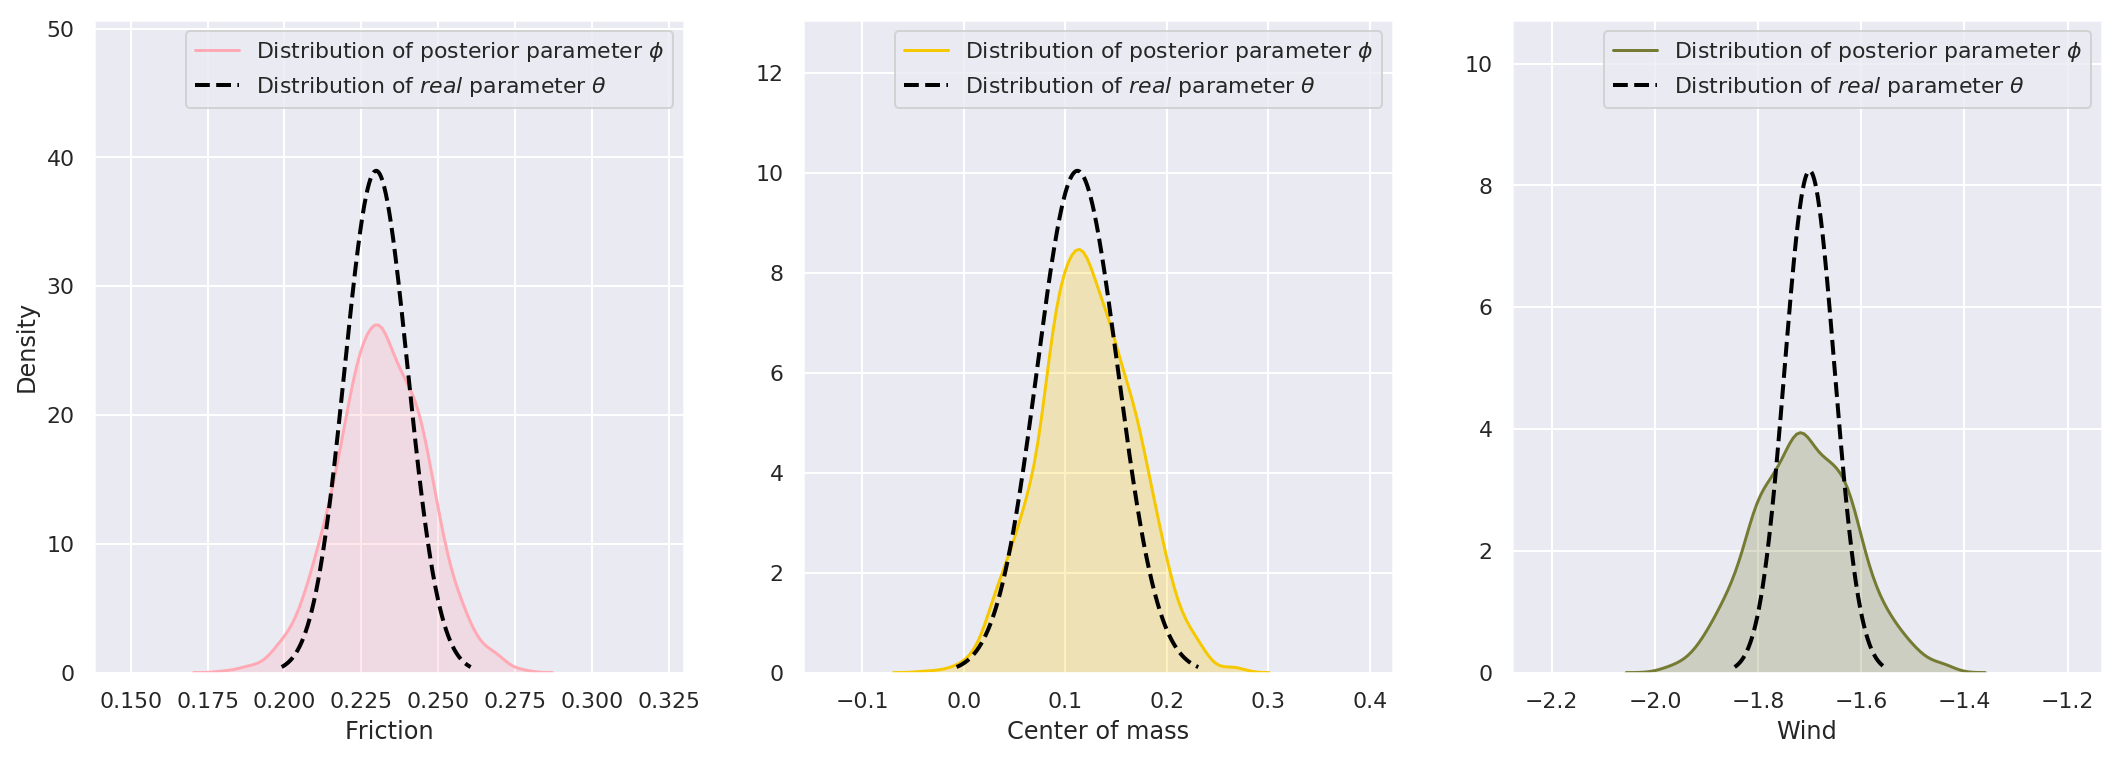
\includegraphics[width=1.0\linewidth]{img/windyslope/latent-representation/new/latent_encoding_iter2}
  \caption{2nd iteration of \dettostoc{}}
\end{subfigure}
\begin{subfigure}{\textwidth}
  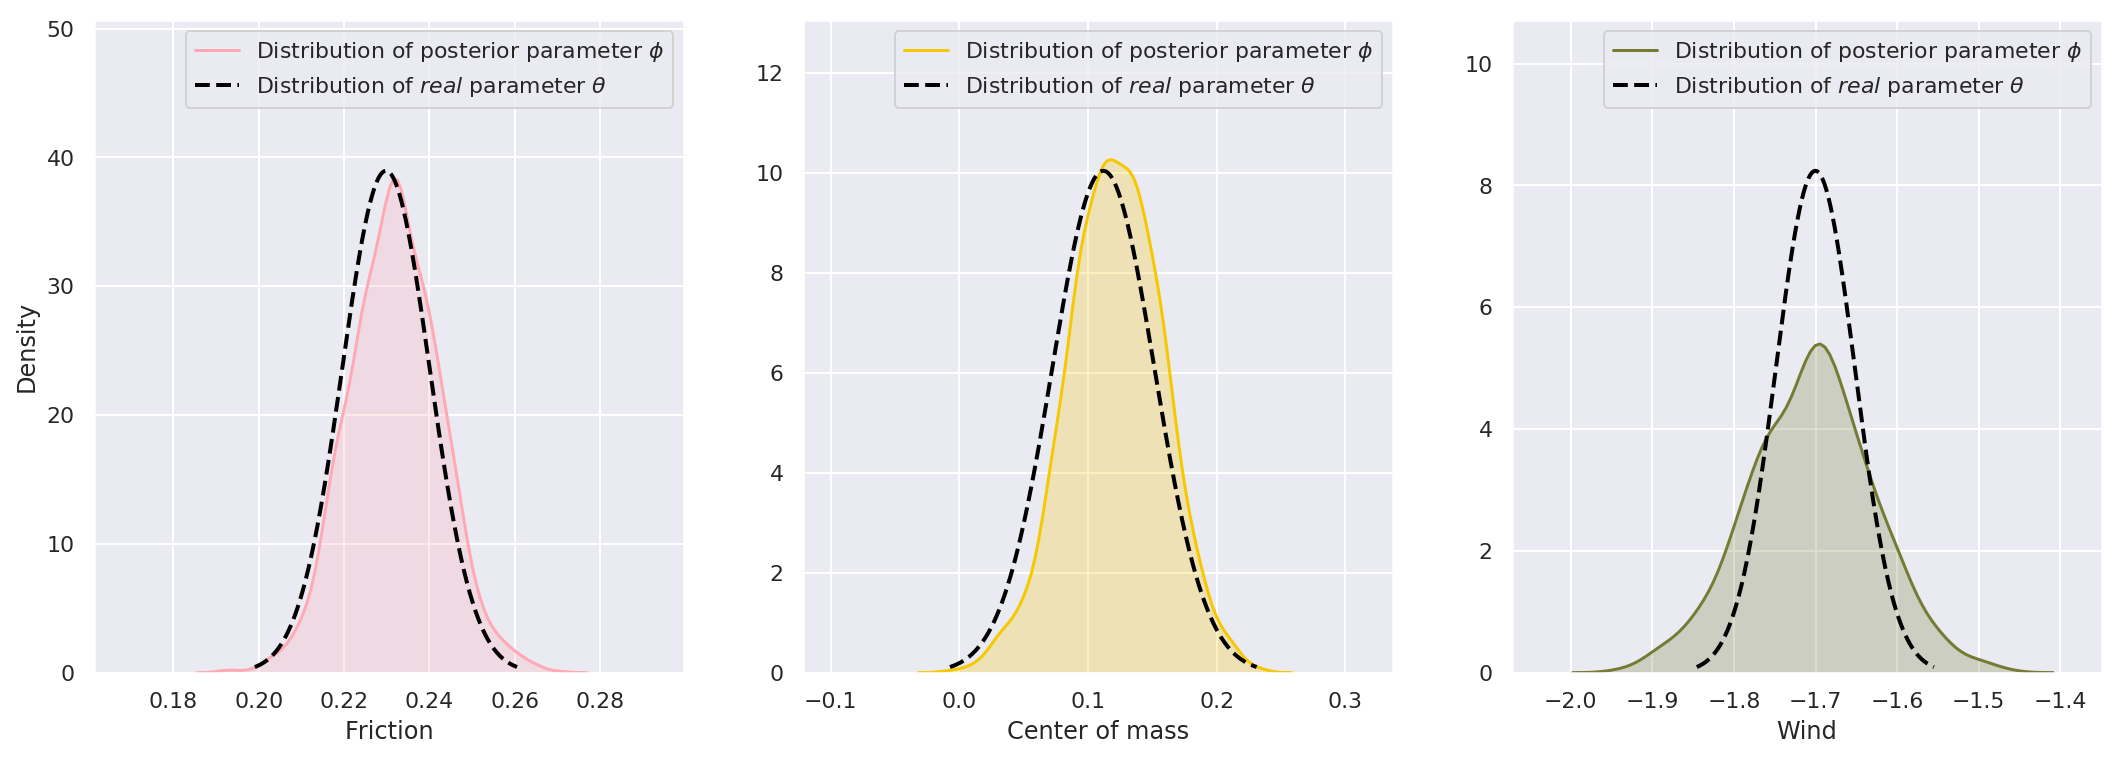
\includegraphics[width=1.0\linewidth]{img/windyslope/latent-representation/new/latent_encoding_iter3}
  \caption{3rd iteration of \dettostoc{}}
\end{subfigure}
\caption{Plots show the learned parameters $\vph_{\mu, \sigma}$ of the posterior given \emph{real} samples $\vec{\xi}^{real}$ as normalized histograms after subsequent steps of \dettostoc{}.
From left-to-right, the latent space codings show tangential friction, center of mass and wind. %The prior parameters $\vpsi$ for each iteration of \dettostoc{} are included for clarity in a lighter color, along with the true distribution $\theta_{\mu, \sigma}$ in black dashes.}
The \emph{real} distribution of the parameters $\theta_{\mu, \sigma}$ in drawn with black dashes.}
\label{fig:windyslope_latent_space_full}
\end{figure}

\begin{figure}
\centering
\text{Latent space encodings for the YuMi scenario.}
\captionsetup{size=footnotesize}
\begin{subfigure}{0.45\textwidth}
  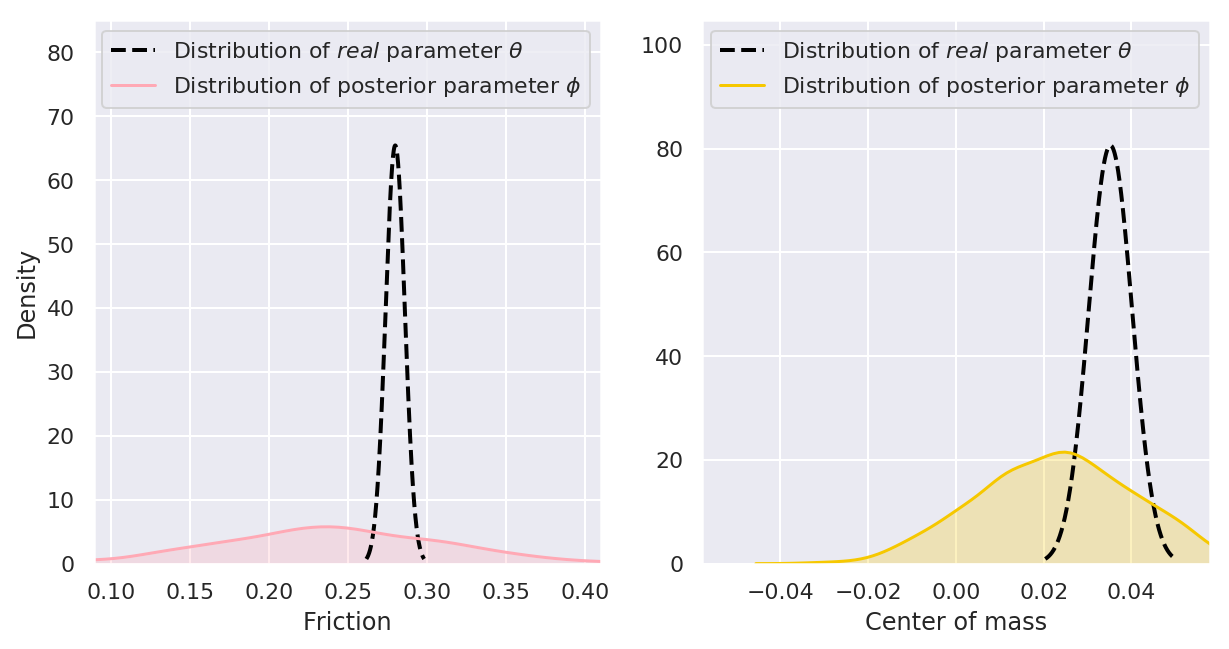
\includegraphics[width=\textwidth]{img/yumi/latent-representation/yumi_latent_encoding_0_iter}%
  \caption{Initial estimates of $\vpsi$ before \dettostoc{}}
\end{subfigure}
\begin{subfigure}{0.45\textwidth}
  \centering
  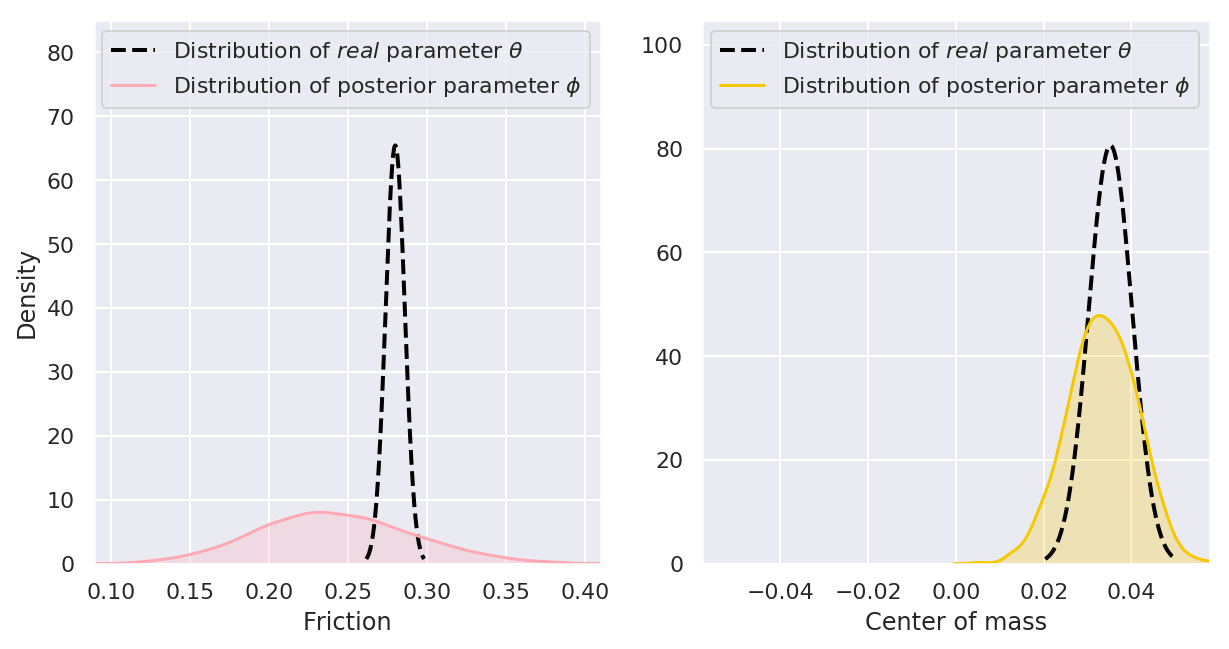
\includegraphics[width=\linewidth]{img/yumi/latent-representation/yumi_latent_encoding_1_iter}
  \caption{$\psi$ after 1st iteration of \dettostoc{}}
\end{subfigure}
\begin{subfigure}{0.45\textwidth}
  \centering
  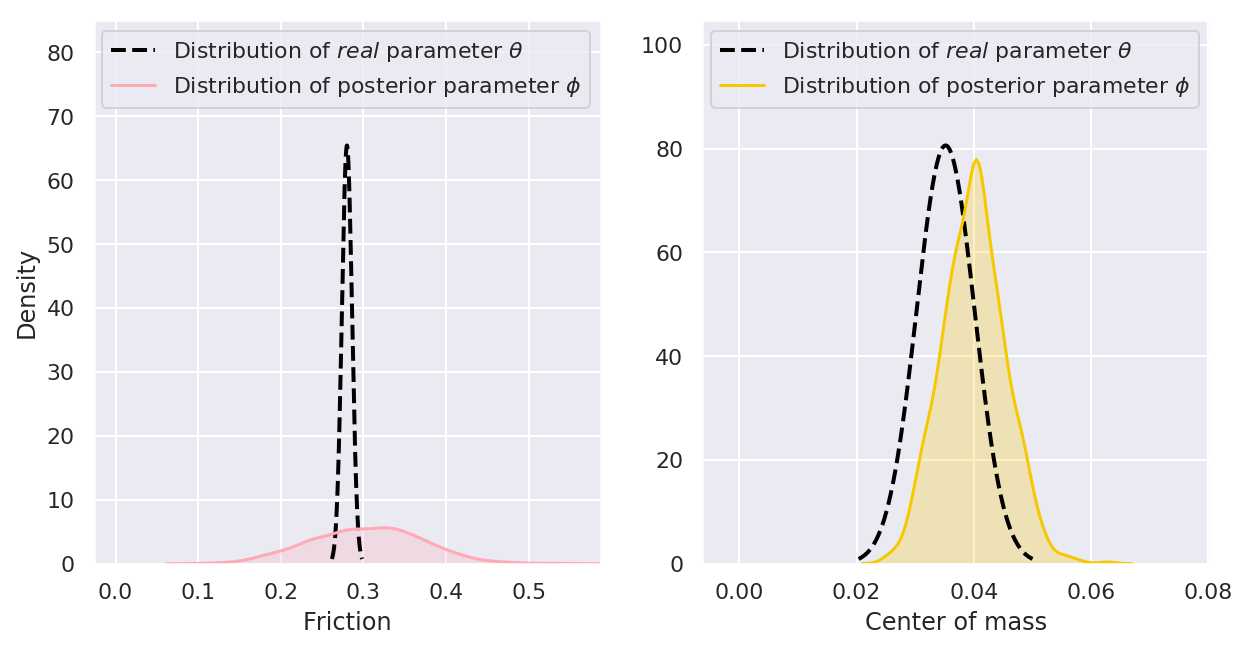
\includegraphics[width=\linewidth]{img/yumi/latent-representation/yumi_latent_encoding_2_iter}
  \caption{$\psi$ after 2nd iteration of \dettostoc{}}
\end{subfigure}
\begin{subfigure}{0.45\textwidth}
  \centering
  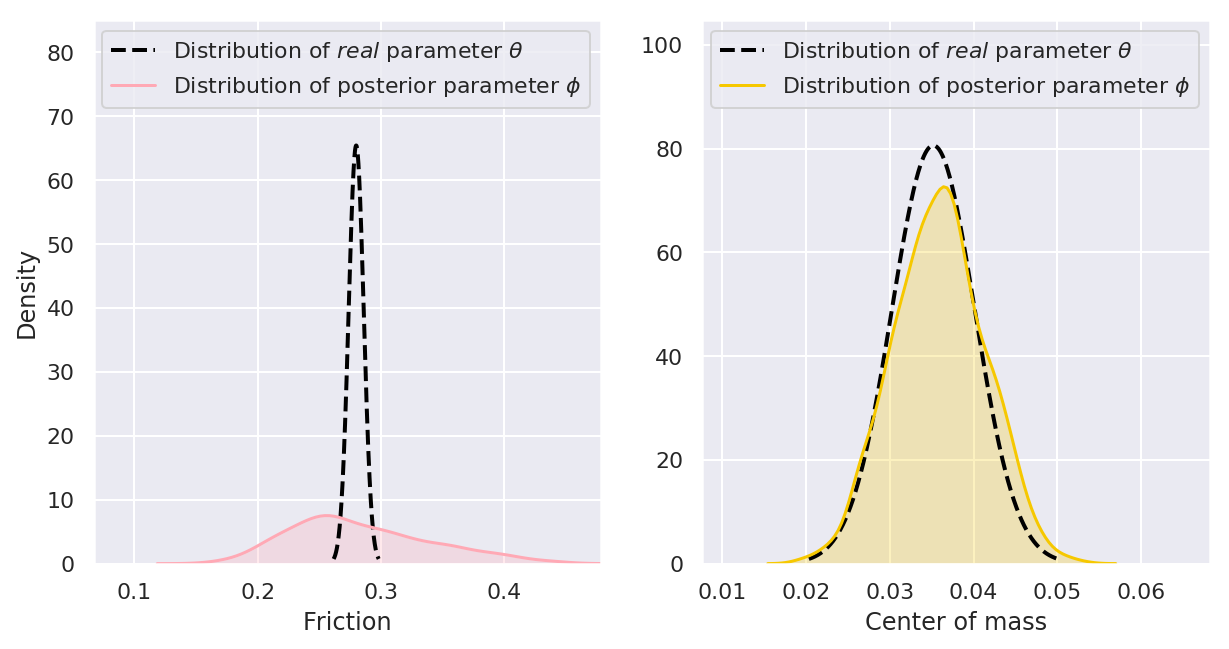
\includegraphics[width=\linewidth]{img/yumi/latent-representation/yumi_latent_encoding_3_iter}
  \caption{$\psi$ after 3rd iteration of \dettostoc{}}
\end{subfigure}
\caption{Plots show the learned parameters $\vph_{\mu, \sigma}$ of the posterior given \emph{real} samples $\vec{\xi}^{real}$ in the YuMi scenario for four iteration of \dettostoc{}.
The parameters correspond (from left-to-right) to tangential friction $\pfriction$, center of mass $\pcom$. The true distributions $\vth_{\mu, \sigma}$ are outlined in black dashes. In this scenario, \dettostoc{} struggles to match $\pfriction{}$ with the true distribution $\th_\textsc{friction}$. This is likely due to the fact that the learned policy pushes the box in small increments, and small changes in friction do not cause any noticeable difference. The posterior for all iterations can be found in the appendix.}
\label{fig:yumi_latent_space_full}
\end{figure}

\begin{figure}
    \centering
    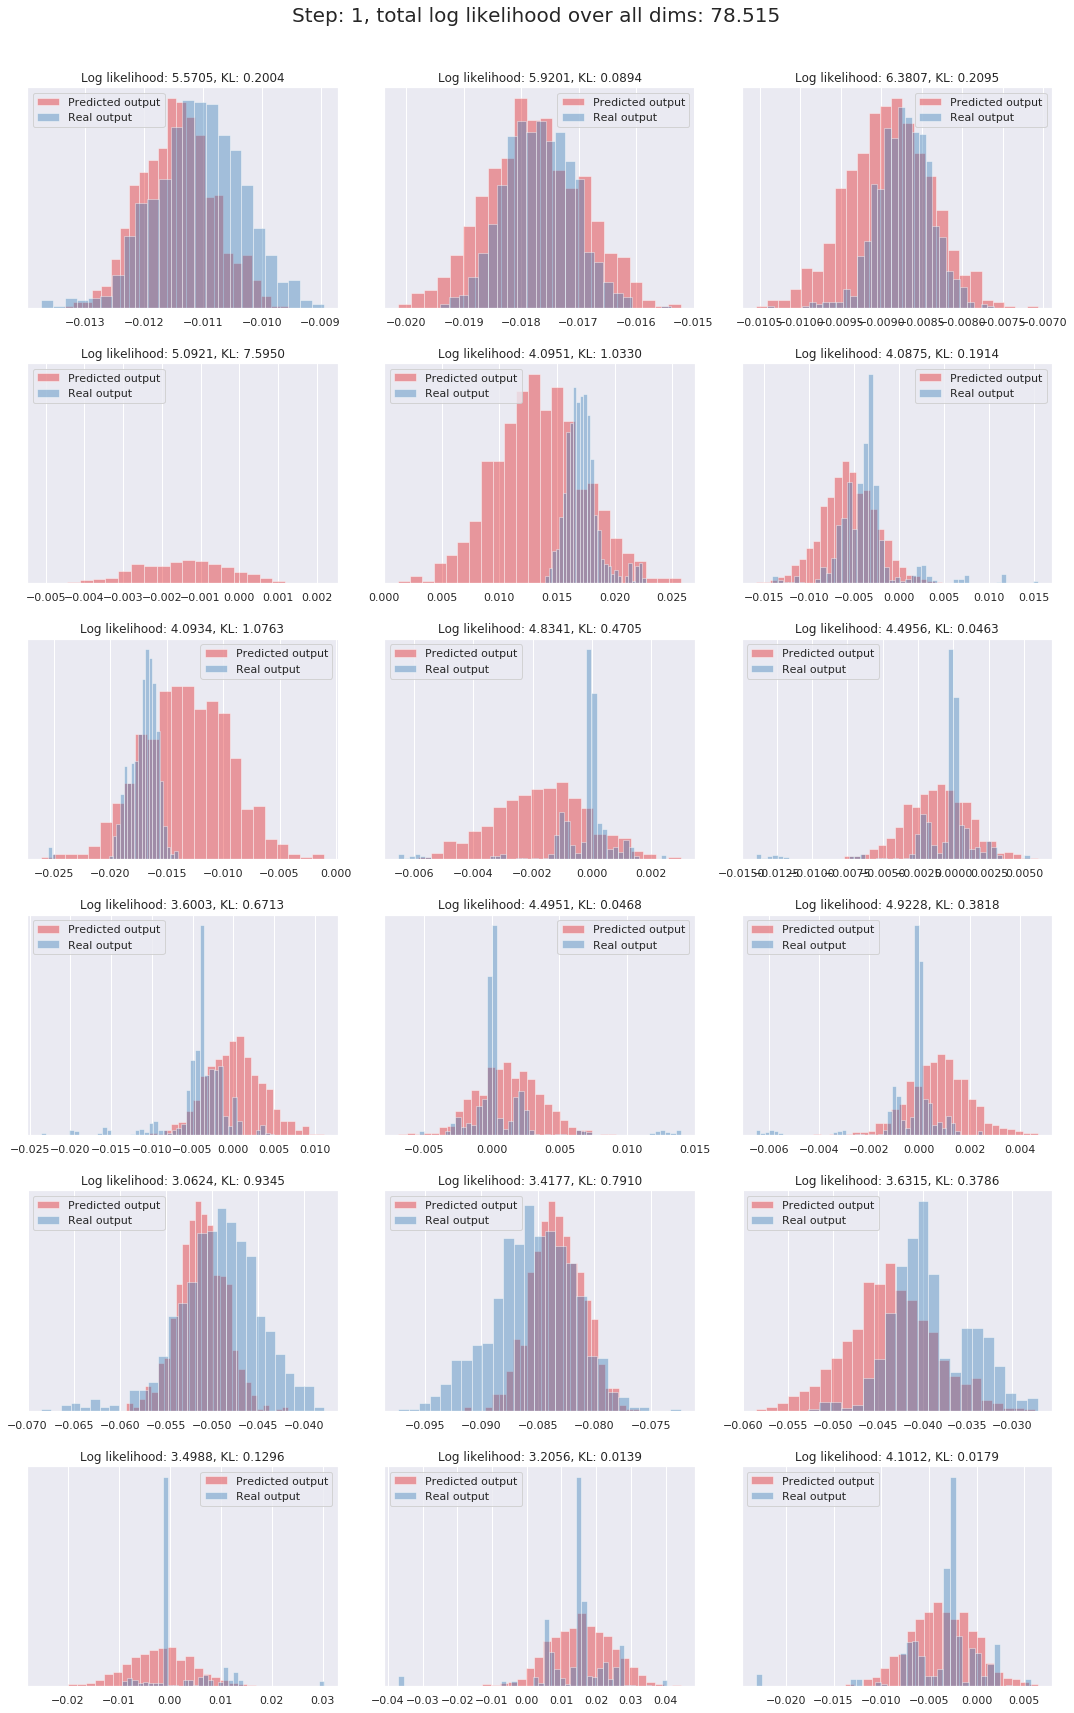
\includegraphics[width=0.8\textwidth]{img/windyslope/output/windyslope_output_det2stoc2_dist_10_step1_iter4.png}
    \caption{Output predictions $\ptheta \protect\given*{\vns}{\vs}$ for a randomly sampled state at $t=1$ for iteration 4 of \dettostoc{}.}
    \label{fig:output_distribution_step1_posvel_dettostoc}
\end{figure}%
\begin{figure}
    \centering
    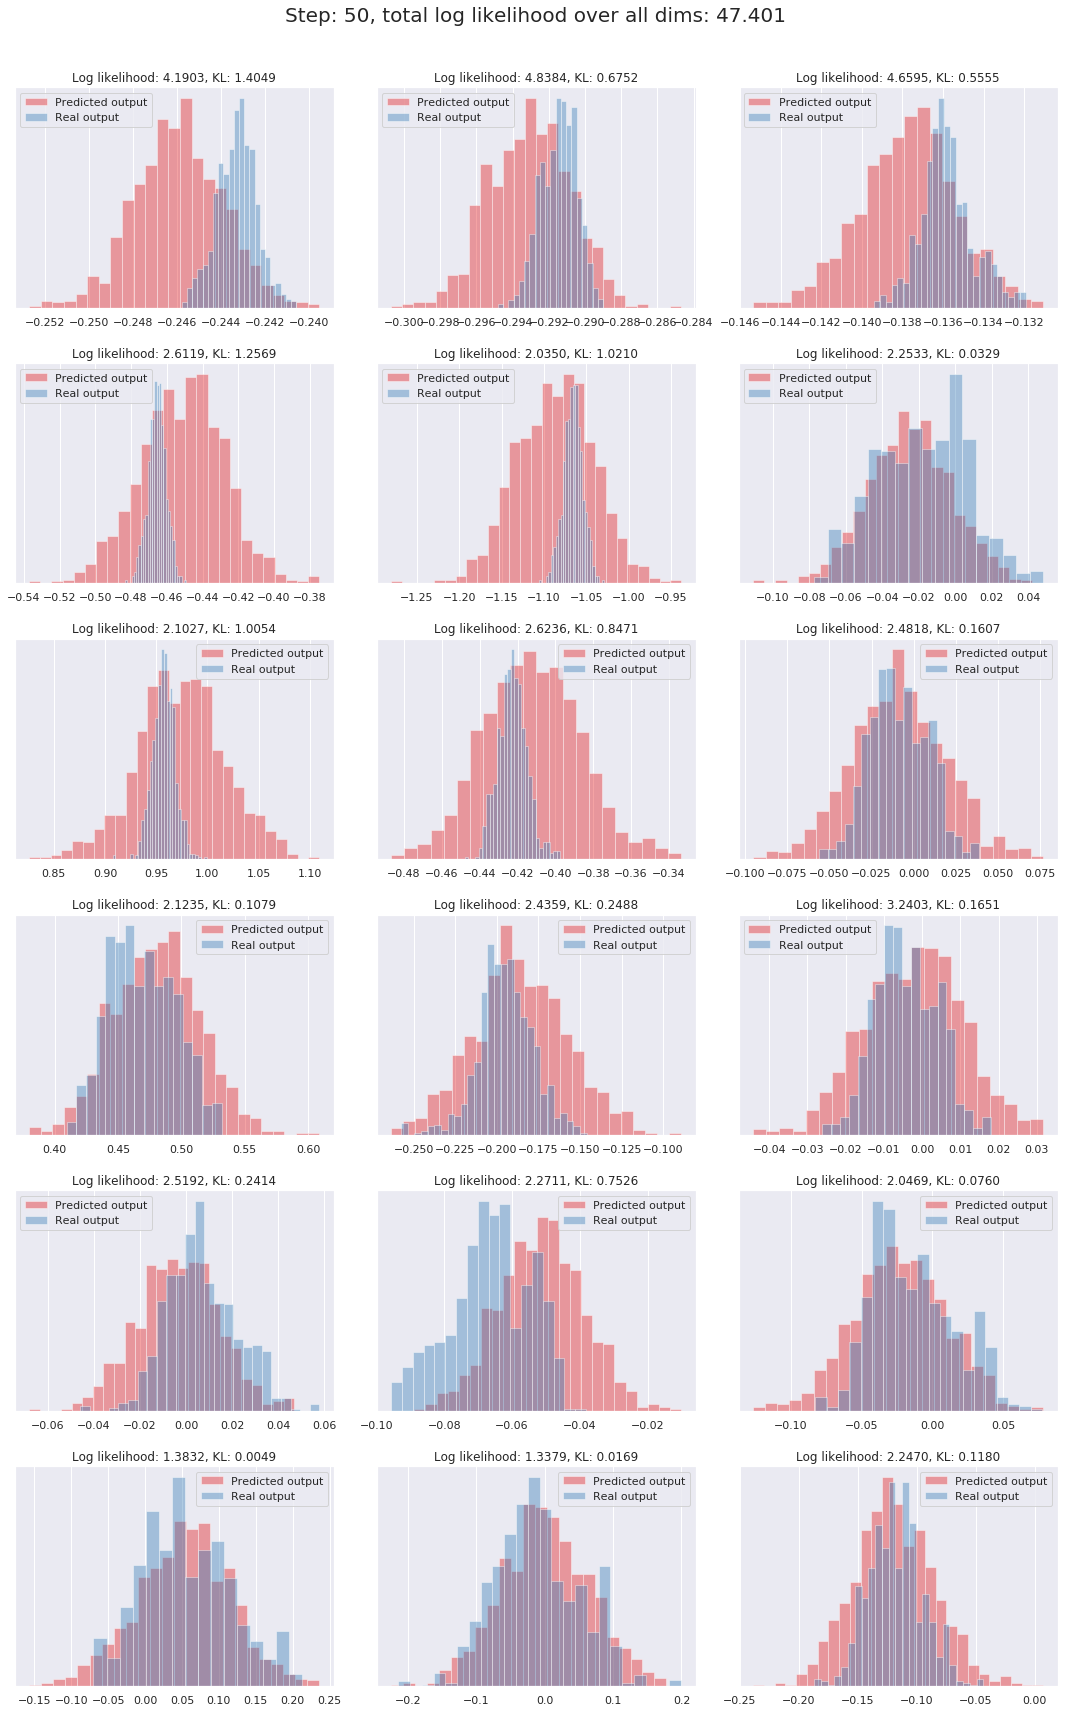
\includegraphics[width=0.8\textwidth]{img/windyslope/output/windyslope_output_det2stoc2_dist_10_step50_iter4.png}
    \caption{Output predictions $\ptheta \protect\given*{\vns}{\vs}$ for a randomly sampled state at $t=50$ for iteration 4 of \dettostoc{}.}
    \label{fig:output_distribution_step50_posvel_dettostoc}
\end{figure}
\begin{figure}
    \centering
    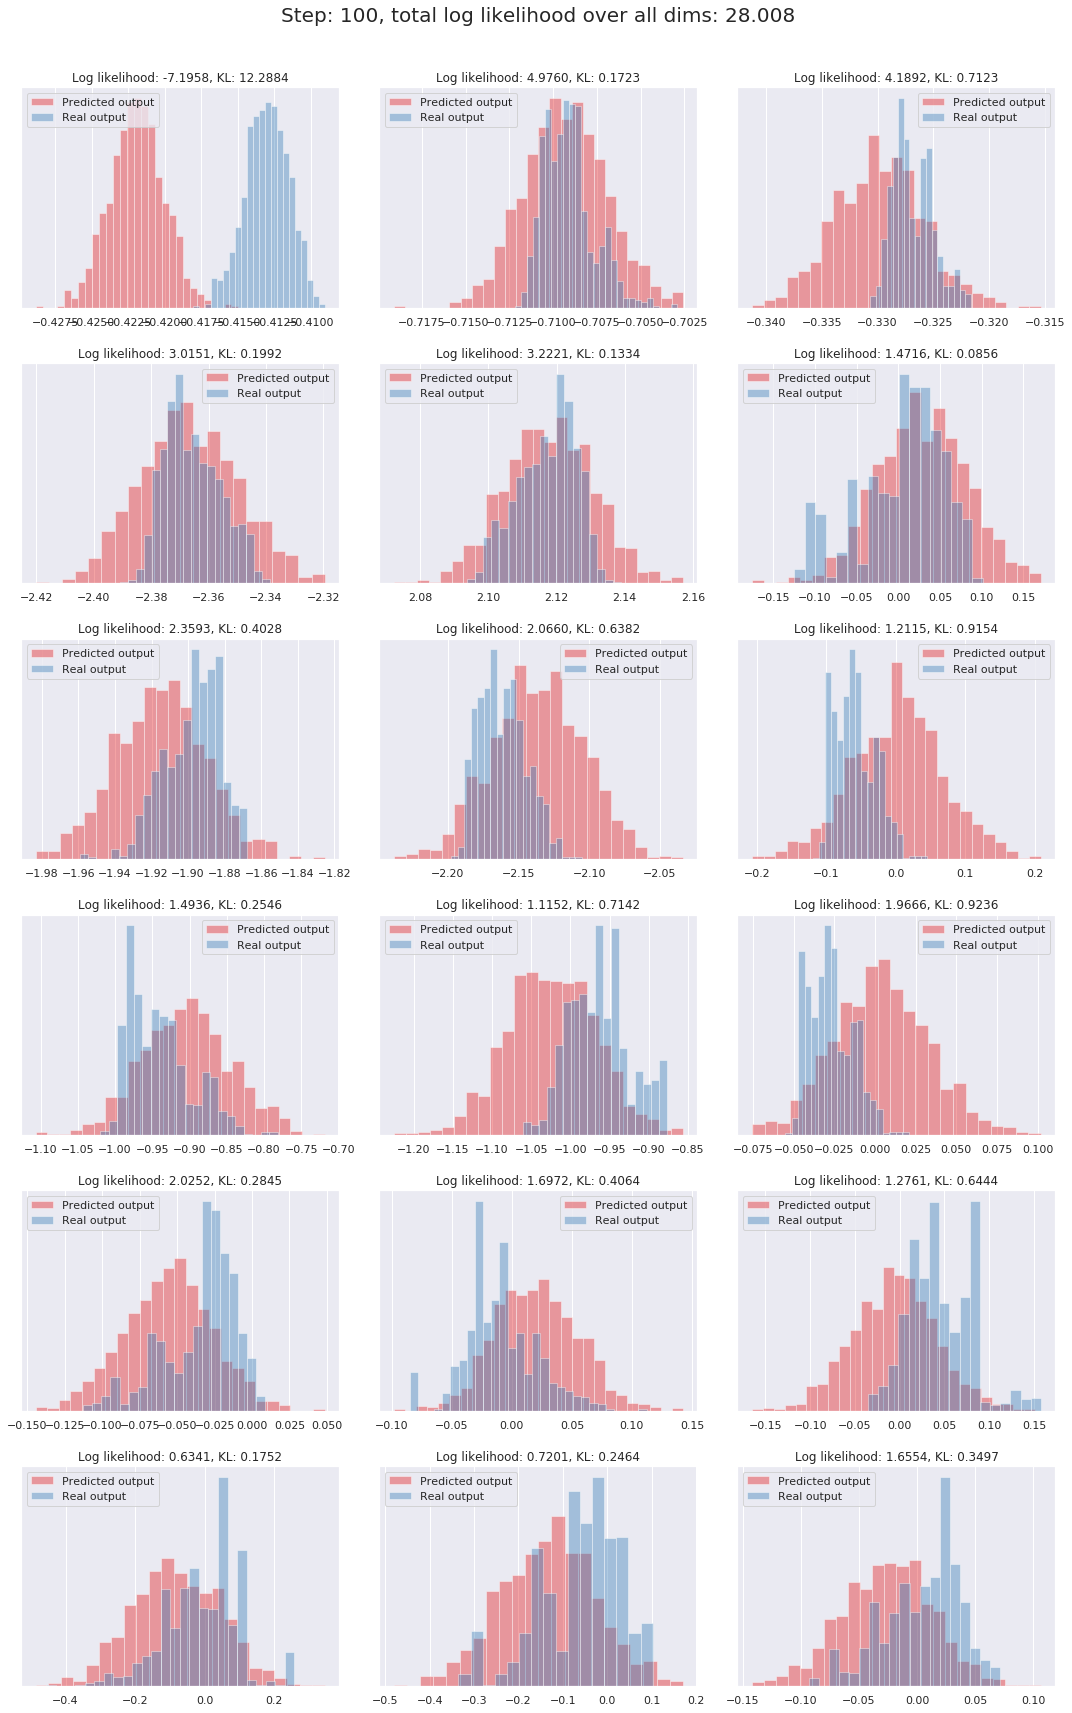
\includegraphics[width=0.8\textwidth]{img/windyslope/output/windyslope_output_det2stoc2_dist_10_step100_iter4.png}
    \caption{Output predictions $\ptheta \protect\given*{\vns}{\vs}$ for a randomly sampled state at $t=100$ for iteration 4 of \dettostoc{}.}
    \label{fig:output_distribution_step100_posvel_dettostoc}
\end{figure}
\begin{figure}
    \centering
    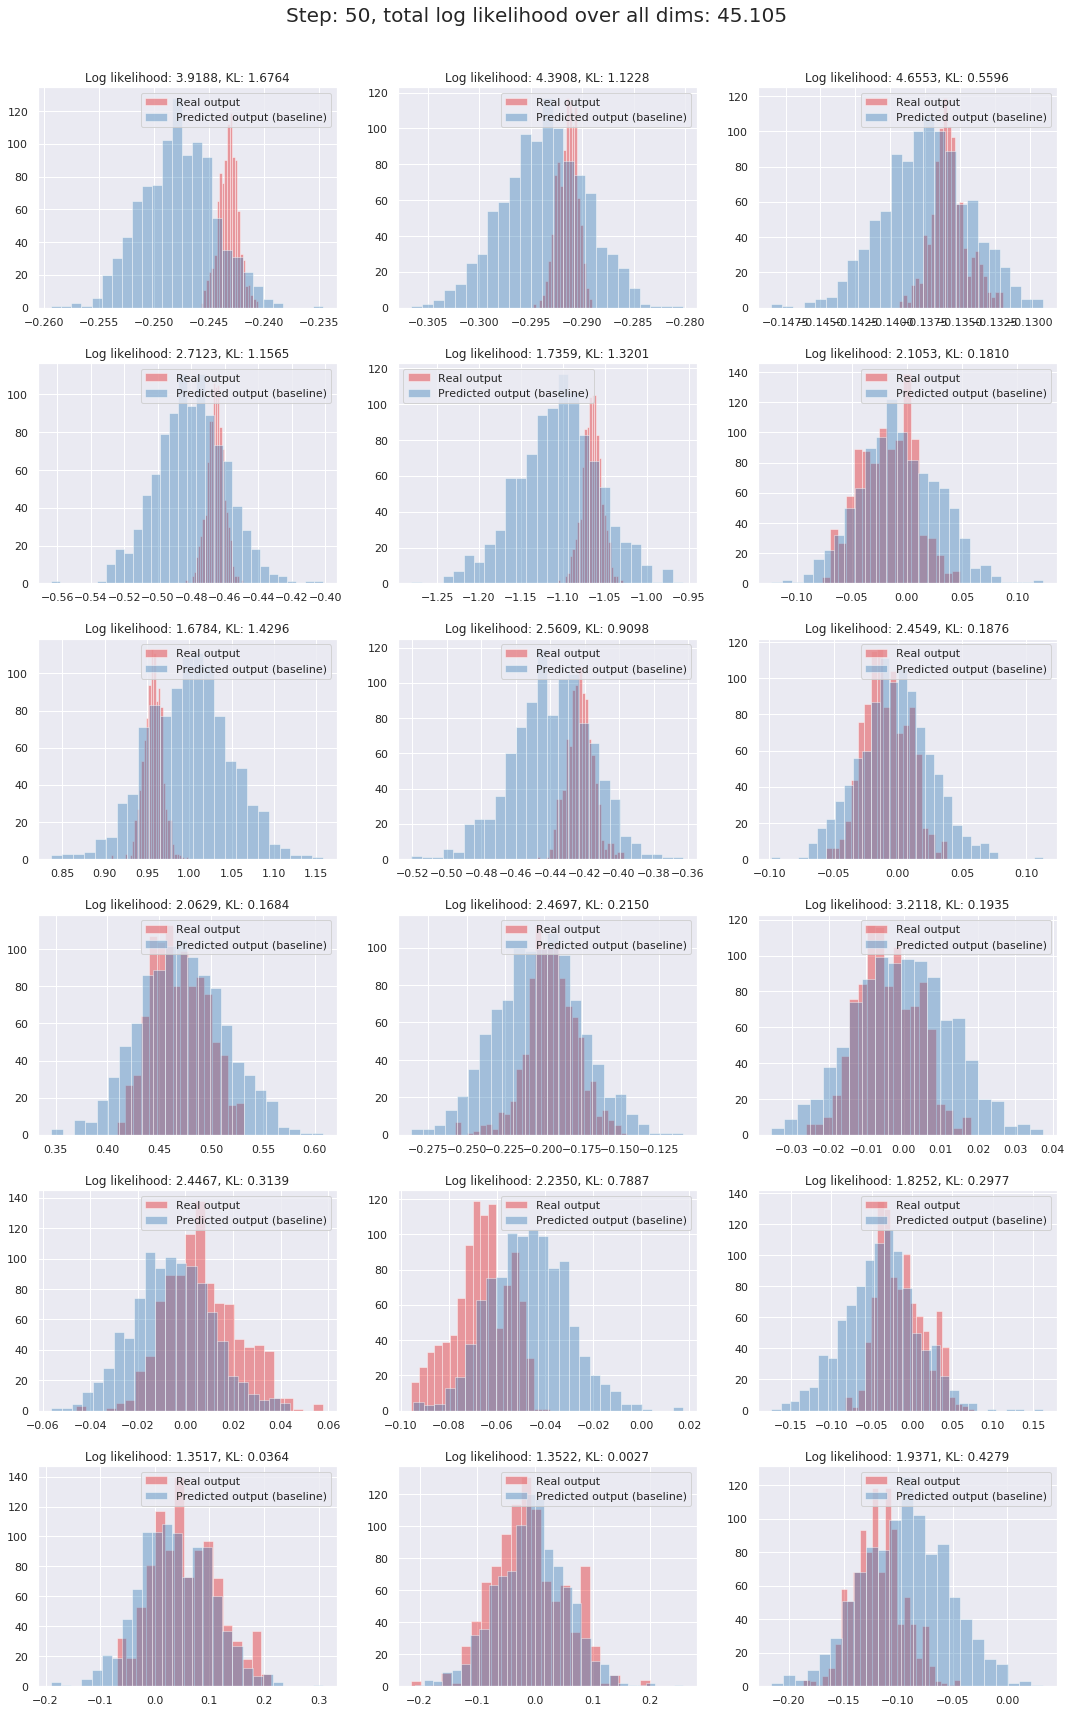
\includegraphics[width=0.8\textwidth]{img/windyslope/output/windyslope_output_baseline_dist_10_step50.png}
    \caption{Output predictions $\ptheta \protect\given*{\vns}{\vs}$ for a randomly sampled state at $t=50$ for CVAE (baseline).}
    \label{fig:output_distribution_step50_posvel_baseline}
\end{figure}

